% ----- formatovani dokumentu -----------------------------------------------
\documentclass[12pt,a4paper,titlepage,final]{report}
\usepackage[utf8]{inputenc}
\usepackage[T1, IL2]{fontenc}
\usepackage{graphicx}
\usepackage{epstopdf}
\usepackage[margin=2cm]{caption}
\usepackage[top=3cm, left=2cm, right=2cm, text={17cm, 24cm}, ignorefoot]{geometry}
\usepackage{color}

% ------ commands -----------------------


% ---------------------------------------

\usepackage{url}
\usepackage{setspace}
\singlespacing
\usepackage[square, numbers]{natbib} 
\pagestyle{plain}
\pagenumbering{arabic}
\setcounter{page}{1}

\setlength{\parindent}{1cm}	
\usepackage{natbib}
\renewcommand{\thesection}{\hspace*{-1.0em}}
\renewcommand{\thesubsection}{\arabic{subsection}}



% ----- vyberte jazyk -------------------------------------------------------
\usepackage[english,czech]{babel}
%\usepackage[english]{babel}

% ----- dopiste titulky -----------------------------------------------------
\newcommand\Course{	Grafická a zvuková rozhraní a normy}
\newcommand\WorkTitle{Aktuální vývoj WebGL}
\newcommand\AuthorA{Pavel Macenauer}
\newcommand\AuthorB{Jan Bureš}
\newcommand\AuthorAEmail{xmacen02@stud.fit.vutbr.cz}
\newcommand\AuthorBEmail{xbures19@stud.fit.vutbr.cz}
\newcommand\Faculty{Fakulta Informačních Technologií}
\newcommand\School{Vysoké Učení Technické v Brně}

\usepackage[
pdftitle={\WorkTitle},
pdfauthor={\AuthorA\AuthorB},
bookmarks=true,
colorlinks=true,
breaklinks=true,
urlcolor=blue,
citecolor=blue,
linkcolor=blue,
unicode=true,
]
{hyperref}


% ----- titulni strana ------------------------------------------------------

\begin{document}
	\begin{titlepage}
	\begin{center}
		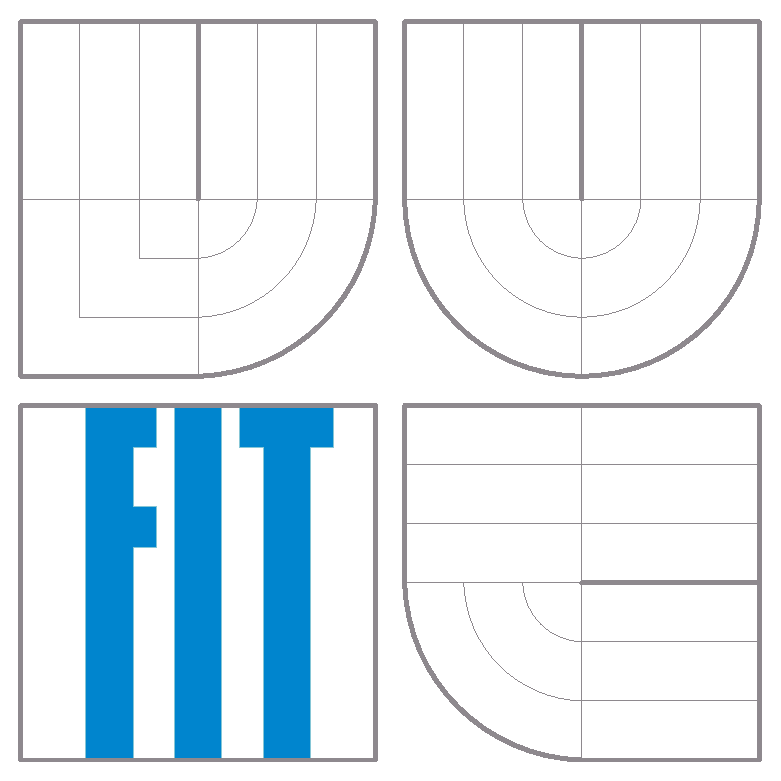
\includegraphics[height=5cm]{images/logo.eps}
	\end{center}
	\vfill
	\begin{center}
		\begin{Large}
			\Course\\
		\end{Large}
		\bigskip
		\begin{Huge}
			\WorkTitle\\
		\end{Huge}
	\end{center}
	\vfill
	\begin{center}
		\begin{large}
			\today
		\end{large}
	\end{center}
	\vfill
	\begin{flushleft}
		\begin{large}
			\begin{tabular}{lll}
				Autor: & \AuthorA, & \url{\AuthorAEmail} \\
				& \AuthorB, & \url{\AuthorBEmail} \\
		
				& & \\
				& \Faculty \\
				& \School \\
			\end{tabular}
		\end{large}
	\end{flushleft}
\end{titlepage}		

	
% ----- obsah --------------------------------------------------------------
	
\tableofcontents

% ----- obsah -------------------------------------------------------------
\newpage
\section{Herní enginy}

Jednou z nejpopulárnějších oblastí, zažívající svůj růst v posledních letech kolem WebGL, jsou herní enginy, technologie a různé další frameworky. Výhodou webu jako platformy pro počítačové hry je, že je závislá pouze na internetovém prohlížeči. Nevyžaduje žádné speciální runtimy, není závislá na operačním systému a není třeba nic instalovat. Stačí pouze otevřít prohlížeč, napsat url adresu a hrát. Jedná se tak o řešení vhodná především pro výpočetně jednodušší úkoly.

\subsection{Přehled používaných knihoven a enginů}

\subsubsection{Construct 2}

Příkladem čeho lze dosáhnout s HTML5 a WebGL je herní 2D editor Construct 2. Nejedná se tak o knihovnu, ale o editor, který již generuje výsledný kód, exportovatelný pro velké množství platforem - HTML5, Chrome, Facebook, Windows Phone nebo i Android či iOS pomocí wrapperů jako CocoonJS.

Nástroj není vhodný pro tvorbu komplexnějších aplikací, spíše jednoduchých her typu Space Invaders, Pac-Man (Pampuch), Tetris. Na druhou stranu nevyžaduje žádnou programátorskou znalost,  je časově nenáročný a hodí se na prototypování.

\begin{figure}[ht]
\begin{center}
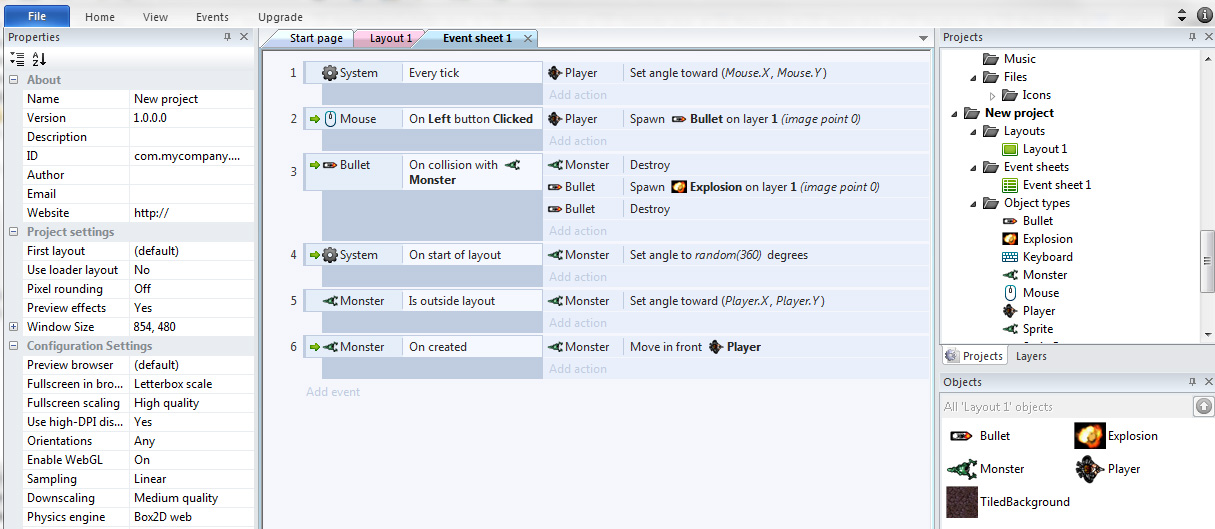
\includegraphics[width=14cm]{images/construct2.jpg}
\caption{Uživatelské rozhraní Construct 2}
\label{fig:theory}
\end{center}
\end{figure}

Při tvorbě aplikace v editoru vytváříte objekty a těm přiřazujete podmínky a následné akce. Nejčastěji se jedná o sprajty, tedy 2D obrázky, ale jako objekty se chovají i vstupní zařízení jako myš nebo klávesnice nebo formulářové prvky. Editor umí pracovata i s AJAXem nebo WebSockets, umožňuje tedy i multiplayer hry a používání databází.

\bibliographystyle{plain}

\nocite{cite1}

\hypertarget{bib}{}
\bibliography{reference}
\addcontentsline{toc}{section}{Literatura}

\end{document}

